\section{Experiments}
\label{sec:experiments}

\begin{figure*}[t]
    \centering
    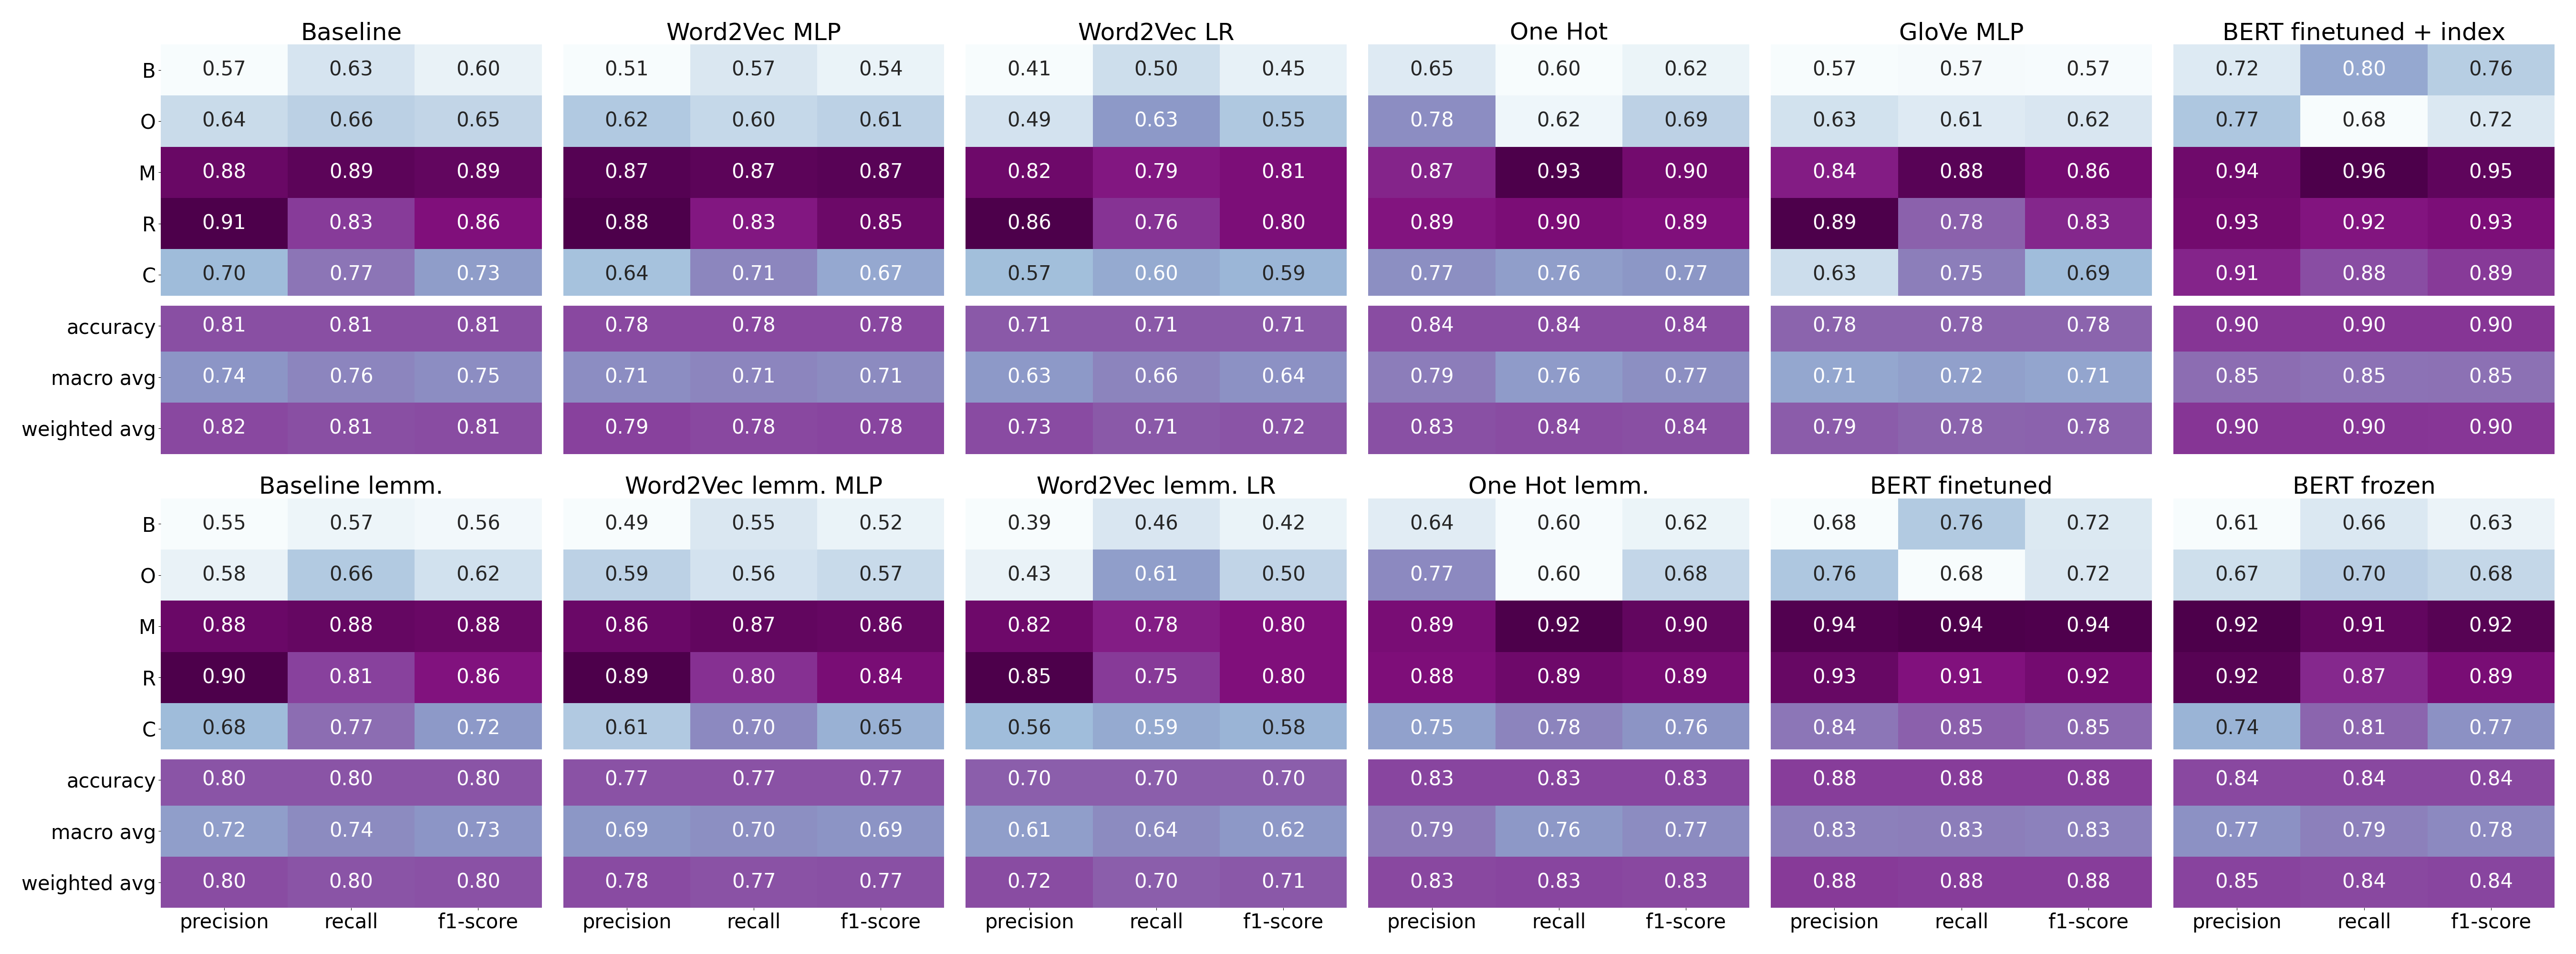
\includegraphics[width=1\textwidth]{figures/classification_report.png}
    \caption{Per-class metrics associated with our model performances on the test set. Only the seed achieving the best performance is shown. The class abbreviations are as follows: 'B' is background, 'O' is objective, 'M' is method, 'R' is result, and 'C' is conclusion.}
    \label{fig:classification_report}
\end{figure*}

\begin{figure*}[t]
    \centering
    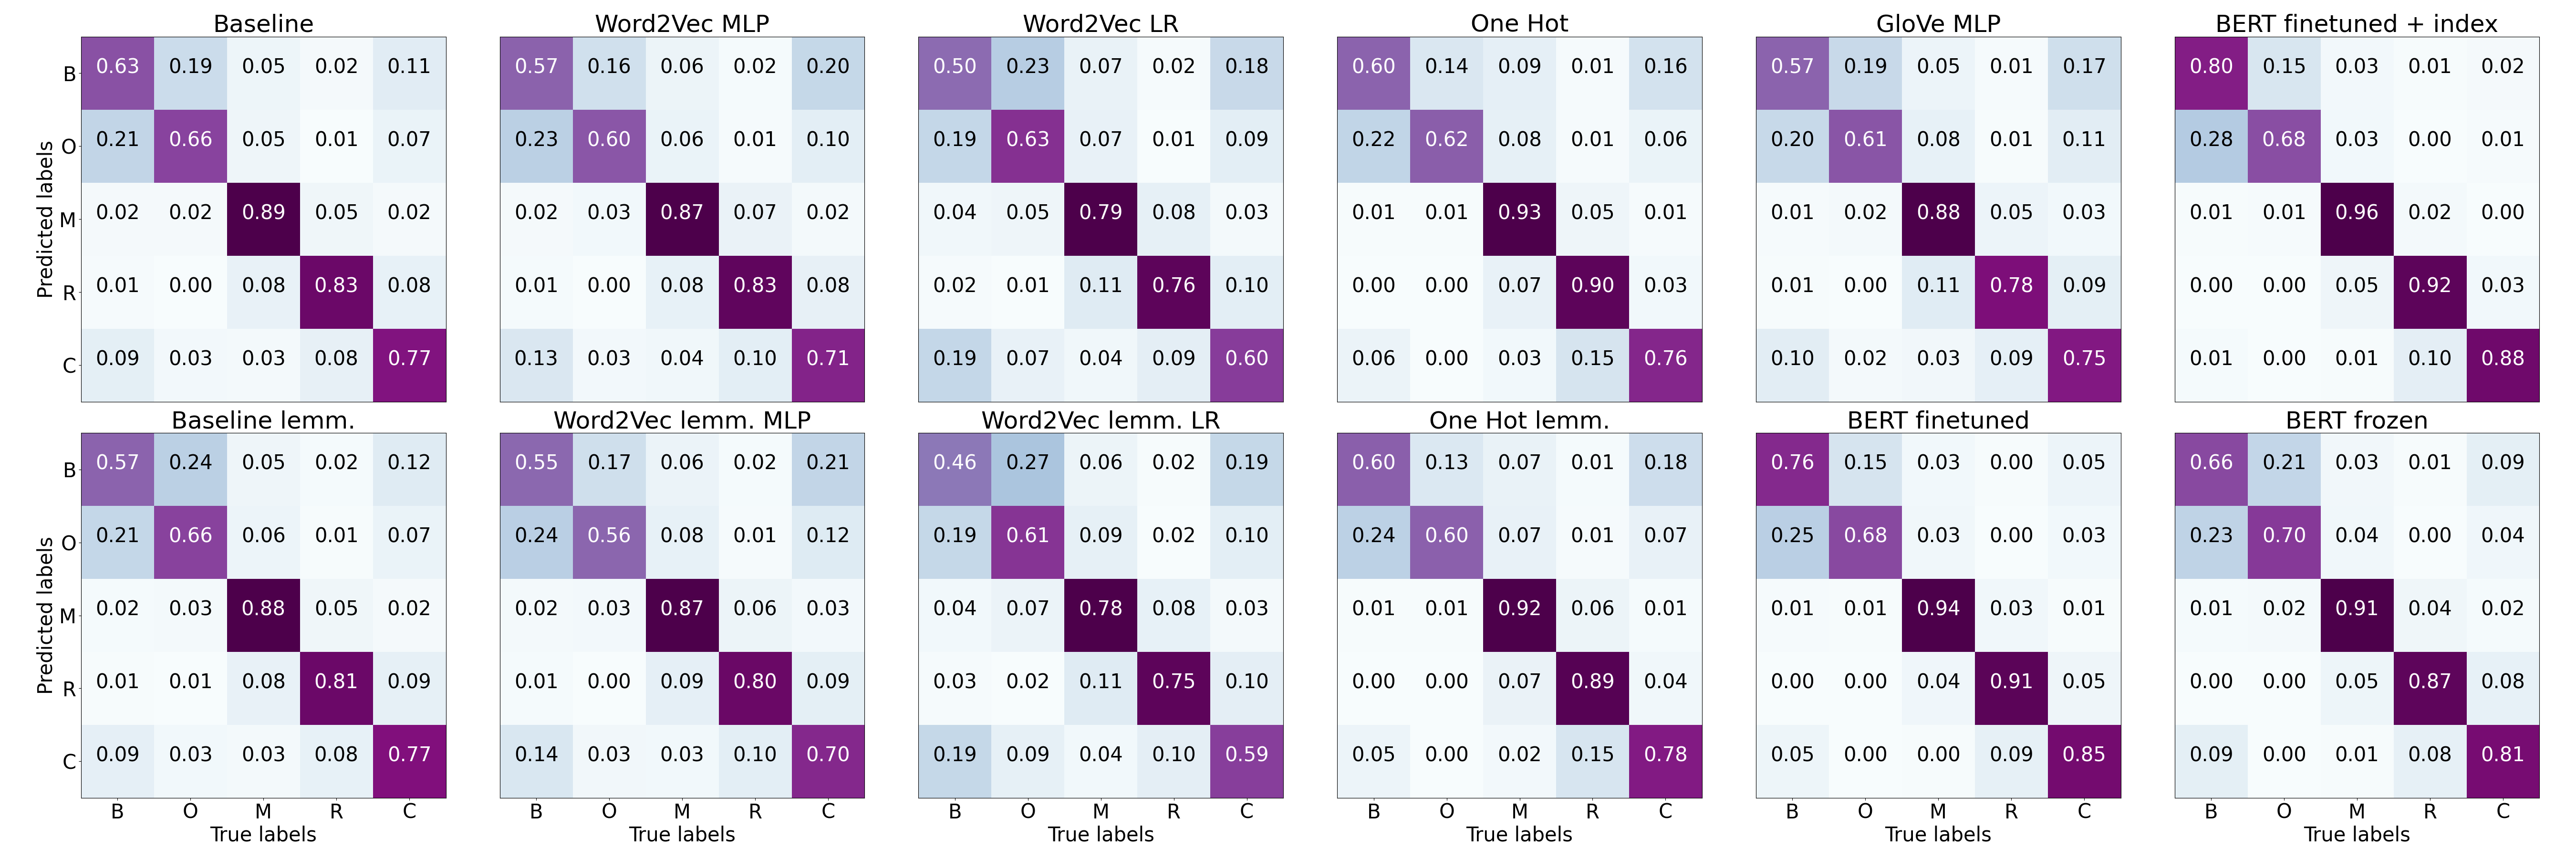
\includegraphics[width=1\textwidth]{figures/confusion_matrices.png}
    \caption{Confusion matrices associated with our model performances on the test set. Only the seed achieving best performance is shown. The class abbreviations are as in \autoref{fig:classification_report}}
    \label{fig:confusion_matrices}
\end{figure*}

\subsection{Experimental Setup}
All of our experiments were performed on the ETH Euler cluster\footnote{\url{https://scicomp.ethz.ch/wiki/Euler}} using 1 unknown GPU and 1 unknown CPU with 32 GB of reserved RAM.% We repeated every model run five times with consecutive seeds (seed 42 to 46) and report the mean and standard deviation.

The baseline models and the logistic regression classifier used in the word embedding model were developed using Scikit-learn \citep{scikit-learn}. Instead of employing a one-versus-rest scheme, we minimize the multinomial loss with L2 regularization for a maximum of 100 iterations using the SAGA optimization method \citep{defazio2014saga} for faster convergence. Preprocessing was performed using spaCy\footnote{\url{https://spacy.io/}} \citep{spacy2020}. For the word embedding models we use the Gensim library \citep{gensim} to train our word2vec model and Tensorflow \citep{tensorflow2015-whitepaper} to develop the MLP trained on top of the word embeddings as well as the one-hot encoded model. We train the models with the Adam optimizer \citep{kingma2014adam} for a maximum of 50 epochs using early stopping. Convergence was assumed when the weighted cross-entropy loss did not improve on the validation set for 3 consecutive epochs. The final models are those with the lowest validation loss. 
% TODO: ADD DESCRIPTION FOR BERT!!! Pytorch citation \citep{pytorch2019}
% TODO: ADD DESCRIPTion FOR GLOVE MODEL! Remember to cite framework used.

Hyperparameters were tuned on a hold-out validation set using extensive random searches \citep{bergstra2012random}. Optimal configurations can be found in the source code. Our final models were trained on the combined training and validation set to further increase performance.

The BERT-based models are trained with AdamW \cite{loshchilov2017decoupled} for 20 epochs with a 12 hour timelimit. Due to the computational cost of BERT, we use common hyperparameters instead of tuning. For \textsc{BERT Freeze} we use a learning rate of 1e-3 while for finetuning BERT we use 3e-5.

\subsection{Results and Discussion}

\autoref{tab:results} shows the weighted F1 scores of the proposed models. We generally observe increasing performance with increasing training time, suggesting a tradeoff between computational cost and performance. As can be seen in \autoref{fig:confusion_matrices} and \autoref{fig:classification_report}, the larger method and result classes are generally predicted more accurately while less frequent classes seem harder to predict and are much more frequently confused with one another.

The TFIDF \textsc{Baseline} performs relatively well, outperforming all word embedding methods. This is surprising given the simplicity of the method. The TFIDF features appear more useful than the more sophisticated word embeddings, especially considering that \textsc{Word2Vec LR} performs much worse than \textsc{Baseline} despite using the same logistic regression classifier. We hypothesize that the semantic information contained in the Word2Vec embeddings is not of high importance for the given task.
Still, the word embedding methods produce useful results. Both, \textsc{Word2Vec MLP} and \textsc{GloVe MLP} yield F1 scores of 0.78. However, we would have expected a more significant performance difference between the domain specific Word2Vec embeddings and the general GloVe embeddings.

The learned Word2Vec embeddings seem to contain interesting relational information about concepts in the medical domain. While we observe no clear trend in \autoref{fig:cause-disease} for embeddings of diseases and their cause, \autoref{fig:treatment-disease} suggests that the differences between diseases and their treatments in the vector space are generally very similar.

Compared to the unsupervised word embedding methods, the \textsc{OneHot} model with the directly learned embeddings performs much better, beating all non-BERT models. However, due to the larger number of parameters, it also takes longer to train. When the corpus is lemmatized the model seems to converge slightly faster and achieves similar performance. For all other methods, lemmatization only seems to hurt performance. Presumably, the word endings provide useful information for the given task.

As expected due to their good general language understanding capabilities, the BERT models outperform all other methods. \textsc{BERT Frozen} performs just slightly better than \textsc{OneHot} but the finetuning yields a significant performance improvement. \textsc{BERT Finetuned + Idx} achieves the best score among all models, however, due to the useful additional input, this comparison is not necessarily fair.

